% To add an image or include a .tex file you need to add
% \CWD
% to the relative (to the main document) path.
%
% Example:
% \begin{figure}
%   \centering
%   \includegraphics{\CWD/images/example.pdf}
% \end{figure}

Maria Joaquina, ou pela alcunha Majô, é uma jovem muito criativa e interessada em ciência. Desde criança, ela aprendeu que o conhecimento racional que a humanidade adquiriu ao longo da história permitiu com que a qualidade de vida melhorasse, e que descobertas ainda maiores fossem feitas. “Coitado dos negacionistas!”, sempre diz ela.

Um dos feitos mais inspiradores para Majô foi a expedição à Lua de 1969, resultado da cooperação de matemáticos, engenheiros e cientistas de várias áreas do conhecimento. Após muito trabalho, o foguete Apollo 11 da NASA levou astronautas de uma base na Terra por uma viagem de 8 dias, com partes muito críticas, como a decolagem, a aproximação e pousos lunares, a operação do módulo lunar, e a reentrada na atmosfera terrestre.

\begin{figure}[!htb]
	\centering
	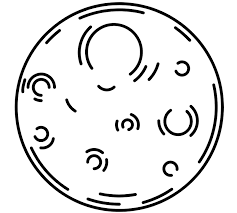
\includegraphics[width=0.2\textwidth]{\CWD/lua.png}
\end{figure}

Nessa viagem, os astronautas Michael Collins, Buzz Aldrin e Neil Armstrong  deixaram um arranjo de espelhos no solo lunar, capaz de refletir raios lasers emitidos a partir do planeta Terra. Quando soube disso, Majô imediatamente começou a montar o equipamento apropriado em seu quintal e chamou todos os seus vizinhos para acompanharem o experimento durante a festa que ela titulou ``AFE – Avoid Flat Earthers''.

Além de conversar sobre astronomia, Majô, amante do estoicismo, também conversará com os convidados sobre outros avanços da humanidade, como o pensamento filosófico, o método científico e as vacinas. Entretanto, para sua surpresa, ela descobriu que vários vizinhos não acreditam na chegada da humanidade à Lua ou em algum avanço da ciência, e vão só causar transtornos em sua festa laser.

Para evitar a fadiga, a jovem Joaquina pediu que você escreva um programa que indica se uma pessoa deve ser cortada do evento, por ser negacionista (``Óbvio, né gente!'', como diz Majô). Neste programa, o vizinho deve informar se ele é negacionista ou não. Se for um pessoa sensata, com certeza será convidada.

\section*{Entrada}

A entrada possui uma linha contendo um valor inteiro $V$, que vale $1$, quando o vizinho analisado é negacionista, e $0$ caso contrário.

\section*{Saída}

A saída possui uma linha com um valor inteiro $A$, que vale $1$ quando o vizinho deve ser convidado por Majô para a festa AFE, de acordo com o critério que ela adota, e $0$ caso contrário.

\section*{Restrições}

\begin{itemize}
	\item $0 \leq V \leq 1$
\end{itemize}


\section*{Exemplos}

\exemplo
